%%%%%%%%%%%%%%%%%%%%%%%%%%%%%%%%%%%%%%%%%%%%%%%%%%%%%%%%%%%%%%%%%%%%%%%%%%%%%%%%
%2345678901234567890123456789012345678901234567890123456789012345678901234567890
%        1         2         3         4         5         6         7         8
% THESIS CHAPTER

% short summary of the chapter
\section*{Summary}
\label{sec:Summary_chap_2}
The objective of this work is to find techniques that might help improve classification and segmentation of SAR images.\newline
Given an image of the radar brightness ($\sigma^0)$ of an area or the image of the coherence between two SAR acquisitions it is possible to segment the image into different areas of interest, for example, given an image of the Amazon Forest someone might be interested in generating a map of the area that was deforested and the area that it is still preserved. \newline
Even though there are many machine-learning algorithms that can do this with an acceptable accuracy, these algorithms are not perfect and have a error that is noticeable. \newline
To improve the result of those algorithms the textures of the image will be analyzed and then it will be validated if it is possible to extract useful information from these textures that otherwise would be hidden to the traditional algorithms for classification, like random forest or neural networks.\newline
In some images, the texture might be a defining feature of a specific region and critical to obtain a correct classification.
The main idea of the looking at the textures of an image is to extract information based not only on the value of intensity of the pixel, but also looking at the pixels that are around that one, such that the value of a texture in a single pixel is a function that depends on the value of the original pixel and the pixels that are nearby it.\newline
The textures are a function of the spatial arrangement of intensities and colors in an image. Even though different images might have the same histograms of pixel intensities, they can be very different, and sometimes, analyzing just the histograms of the pixel intensities might not be enough to define in which region a pixel is in. There are two main approaches to analyze the textures of an image: the structural approach and the statistical approach. In this work it will be only used the statistical approach for analyzing textures.

\section{Machine Learning and the problems for classification}
\label{sec:machine_learning_problems}
Machine Learning is one of the most important and influential technologies in today's world. It is also one of the areas that has the most focus on research since the demand is very high, therefore it is very likely that there is still much room for improvement and its full potential has not yet been reached. \newline
Machine learning is a tool that was developed to deal with the excessive amount of data that has started to appear from 50 years ago until now. But this excessive amount of data is useless if there is no way to extract useful information from it. Focusing on this problem, machine learning is a field of study that tries to analyze data and find the hidden patterns hidden within it. Finding these patterns might be useful to make predictions of a problem and even help taking decisions on how to act when presented a situation.\newline
The name machine learning comes from the fact that the algorithms have to go through a learning process, trying different rules and seeing how well they perform to describe the problem presented. Among the different forms of machine learning, on this work there will be a focus on the supervised machine learning, which is a type of machine learning system that is presented with data which is labeled, that means that each data has a correct label. The goal of this machine learning is that when presented with new data it is possible to predict in which label that data fits. \newline

The are five steps to this process: Data collection, data preparation, model fitting, model evaluation and parameter tuning.
\begin{enumerate}
    \item Data collection: Collect the data the algorithm will learn from (in this case it is the SAR image)
    \item Data preparation: Format the data into optimal format for the algorithm.
    \item Training: The stage in which the algorithm derives a model by fitting the output and the input using some method.
    \item Evaluation: Check how well the algorithm performs
    \item Parameter Tuning: Tune the parameters to improve performance
\end{enumerate}{}

The types of Supervised learning are two: Classification and regression.
\begin{enumerate}
    \item Classification: The output is a category, like a color, or in the case of a SAR image, if the pixel indicates a area of forest or a deforested area.
    \item Regression: The output is a real number, such as height or price.
\end{enumerate}{}

On this work, classification machine learning will be used to classify a SAR image into regions of forest and deforested areas. \newline
There are several machine learning algorithms, such as: C-support vector classifier, K-nearest neighbors classifier, multi-layer perceptron, Gaussian process classification, Radial-basis function kernel, Decision tree classifier, AdaBoost classifier, Random forest classifier, Gaussian Naive Bayes classifier, Quadratic discriminant analysis classifier and neural network classifier.\newline

All those different algorithms try to solve the same problem: given a set of input labeled data, what is the model that best fits the labeled input data and the given label, in order to predict labels for unlabeled data with least error?\newline
The difference between those algorithms is that the model that each one will find is different. Some algorithms, like the neural network, will try to derive a model using linear functions on the input data and trying to minimize the mean square error(MSE) between the predicted output and the label for example, as the decision trees for example will try to create a series of binary questions and by combining the answers of these questions will give the label of the input data.
\newline
Either way, the model of each algorithm can be geometrically understood by creating decision regions in a $R^n$ space ($n$ is the number of input variables), and by looking in which region a input is located, it is possible to give the output answer.
\newline
For example, if the number of input variables is 2, and different algorithms are run to classify labeled data between two colors (blue and red) the result can be seen in the figure below.

\begin{figure}[H]
    \centering
    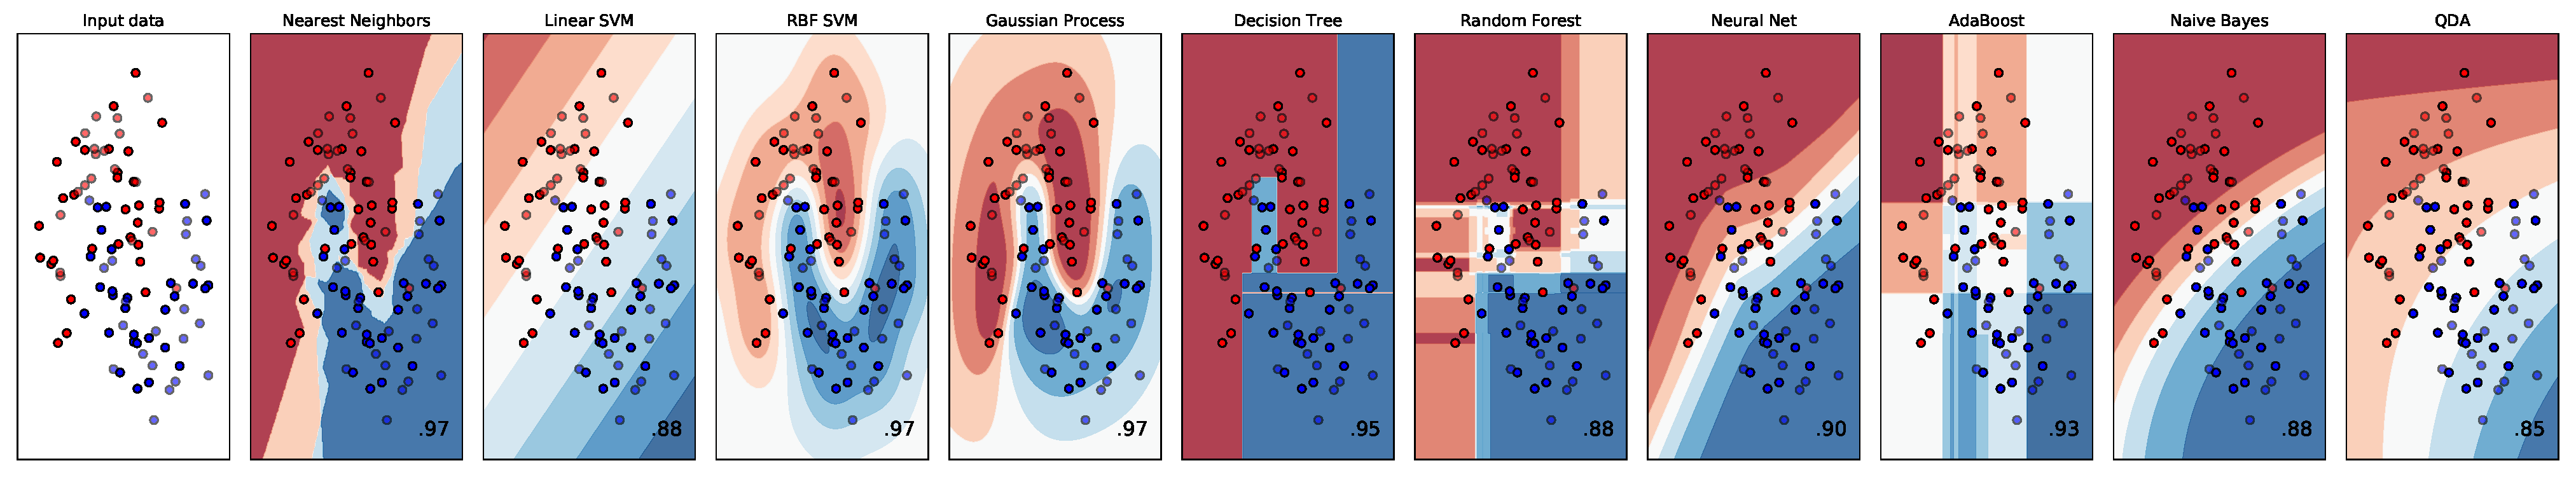
\includegraphics[width=\linewidth]{Chapter3/regions.pdf}
    \caption{Classification Boundaries for Different Algorithms.}
    \label{fig:machine_learning_classification}
\end{figure}{}

In \figref{fig:machine_learning_classification}, the color intensity illustrates how certain the algorithm is of the classification and the number on each figure is the time it took to create that region.
\newline
For different algorithms it is clear that the classification regions it derives are different and how the algorithm creates these regions determines how well the algorithm classifies.
\newline
The problem of using machine learning for classifying forest and deforested areas is that the algorithm relies too much on creating decision boundaries and by checking in which decision region a certain pixel is, but it does not check the surroundings of that pixel, which is also a important information for classification. \newline
\newline
For example, in \figref{fig:machine_learning_classification}, if a red pixel falls in a blue region it will be wrongly labeled blue. For a SAR image it might happen that due to noise a forest pixel looks like a deforested pixel, but if all the pixels around it looks like forest pixels then this might be an indicator that that pixel is a wrongly labeled forest pixel. Even though it is not possible to make these machine learning algorithms consider this question in the learning process (this would mean interfering  in the modelling process, which would be equivalent to creating a new algorithm), it is possible to create more input data by looking at the surroundings of a pixel. This new data information can help this algorithm not to make a wrong classification. This new input data is exactly the textures of a image.

\section{Textures Methods}
\label{sec:Texturization_Methods}
As previously mentioned, the textures might give useful information for classification because sometimes the neighborhood of a pixel also provides valuable information for the classification. In forest landscapes, for example, the texture value might depend on the size and distance between trees, such that in high-resolution images if two pixels fall in the same tree then they will have similar value, resulting in a small local variance of intensities, something that will be indicated by the texture value. According to \cite{Woodcock} if the resolution is increased to a size comparable to the size to of trees, then the local variance also increases, something noticeable in tropical forests with a high species diversity. Therefore is important to mention that the texture is dependent of the resolution of the image, and the texture of a high resolution image of an area might be different than a low resolution image of the same area.

On this work it will be used three different textures methods for improving classification results: the Grey level co-occurrence matrix(GLCM) method, the Laws textures method and the sum and different histograms methods.

\section{The GLCM Method}
\label{sec:GLCM_Method}

The first method of texture creation is the grey-level-co-occurrence matrix method.
A co-occurrence matrix is a matrix extracted from an image in which the values in the rows and columns of this matrix represent the set of possible grey scale values of the image. 
For example, the co-occurrence matrix $C$ is a matrix in which the elements represent the possible co-occurrence of values for the image $I$ given a spatial relationship on a set of possible values $V$. 
For example, given a image, the co-occurrence matrix $C$ indicates how many times the value $i$ co-occurs with the value $j$ given a spatial relationship. 
This spatial relationship is given by a displacement vector $d = (d_r, d_c)$ that dictates the distance of the pixels that one wants to analyze the co-occurrence of values.
A more mathematical way to express this matrix is given by the following definition:

\begin{equation}
    C_{d}(i,j) = \# \{(r,c) | I(r,c)=i\  \textit{and} \  I(r+d_r, c+d_c)=j \} 
\end{equation}

For example, if the grey scale image $I$ is equal to:

\begin{equation}
I=
    \begin{bmatrix}
    1&1&0&0\\
    1&1&0&0\\
    0&0&2&2\\
    0&0&2&2
    \end{bmatrix} 
\end{equation}{}


Then three co-occurrence matrices for different displacement vectors $d=(0,1)$, $d=(1,0)$ and $d=(1,1)$ are:
\begin{equation}
    C_{(0,1)}=
    \begin{bmatrix}
    4&0&2\\
    2&2&0\\
    0&0&2
    \end{bmatrix}
\end{equation}{}

\begin{equation}
C_{(1,0)}=
    \begin{bmatrix}
    4&0&2\\
    2&2&0\\
    0&0&2
    \end{bmatrix}
\end{equation}{}

\begin{equation}
C_{(1,1)}=
    \begin{bmatrix}
    2&0&2\\
    2&1&1\\
    0&0&1
    \end{bmatrix}
\end{equation}{}

In $C_{(0,1)}$ the position $(0,0)$ equals 4, which means that $j=0$ appears to the right of $i=0$ four times in the image. The position $(1,0)$ equals 2 because $j=0$ appears to the right of $i=1$ two times in the image. The position $(2,1)$ equals 0 because $j=1$ never appears to the right of $i=2$.

From this grey level co-occurrence matrix it is important to generate the \textit{normalized} grey level co-occurrence matrix $N_d$ given by:

\begin{equation}
\label{eq:normalized}
    N_d(i,j) = \frac{C_d(i,j)}{\sum_i\sum_j C_d(i,j)}
\end{equation}
Co-occurrence matrices capture the texture properties, but are not directly useful for further analysis, such as comparing different textures. To solve this problem, is possible to compute numeric features from this normalized co-occurrence matrix that might give useful information of the image that otherwise would be hidden for machine learning classification algorithms. These numeric features computed from the normalized co-occurrence matrix represent more compactly the textures of the image.
The following textures are features that can be obtained from normalized co-occurrence matrix:
\begin{table}[H]
\centering
\begin{tabular}{ |c |c |}
 \hline
 Contrast & $\sum_{i,j=0}^{N-1} i\frac{N_d(i,j)}{1+(i-j)^2}$\\ 
 Dissimilarity & $\sum_{i,j=0}^{N-1} i N_d(i,j)|i-j|$\\
 Homogeneity & $\sum_{i,j=0}^{N-1}\frac{N_d(i,j)}{1+|i-j|}$\\
 Angular\ Second\ Moment & $\sum_{i,j=0}^{N-1} i N_d(i,j)^2$\\
 Correlation & $\sum_{i,j=0}^{N-1}\frac{(i-\mu)(j-\mu)N_d(i,j)}{\sigma^2}$\\
 Energy & $\sum_{i,j=0}^{N-1}N_d(i,j)^2$\\
 Entropy & $ -\sum_{i,j=0}^{N-1}N_d(i,j)\log_2(N_d(i,j))$\\
 \hline
\end{tabular}
\caption{Formula for texture calculations for GLCM Method}
\label{table:glcm_calculations}
\end{table}

Where $\mu$ is the GLCM mean and $\sigma$ is the standard deviations of the GLCM given by:

\begin{equation}
    \mu=\sum_{i,j=0}^{N-1}iN_d(i,j)
\end{equation}
\begin{equation}
    \sigma^2=\sum_{i,j=0}^{N-1}N_d(i,j)(i-\mu)^2
\end{equation}

A question that rises from this method is how to choose the displacement vector $d=(d_r,d_c)$ such that the result is the best. A solution proposed by  \cite{Zucker} is to run a hypothesis test to check the displacement vector $d$ that most rejects the hypothesis that the pair of pixels separated by the displacement vector $d$ are independent, therefore accepting the hypothesis that this pair of pixels give the most information one of the another and are better suited to compute a texture feature.
The hypothesis test suggests  to run a $\chi^2$ statistical test to find the value $d$ that give the most information, that is, to maximize the value:
\begin{equation}
    \chi^2(d) = (\sum_i\sum_j \frac{N_d^2(i,j)}{\sum_jN_d(i,j)\sum_iN_i(i,j)} -1)
\end{equation}

\section{The Laws Textures}
\label{sec:Laws_Textures}

A different way to create textures is to use 2D filters to detect different kinds of textures. Laws developed a method to measure the amount of variation of the image on a fixed sized window. The method consists of making 16 different convolutions of the original image with convolution masks and use the result to compute the texture. The 16 different filters are obtained by taking the product of the following vectors.
\begin{align}
L5 (Level) = 
\begin{bmatrix}
1&4&6&4&1
\end{bmatrix}\\
E5 (Edge) = 
\begin{bmatrix}
-1&-2&0&2&1
\end{bmatrix}\\
R5 (Ripple) = 
\begin{bmatrix}
-1&0&2&0&-1
\end{bmatrix}\\
S5 (Spot) = 
\begin{bmatrix}
1&-4&6&-4&1
\end{bmatrix}
\end{align}

Then the 2D convolution masks are obtained by taking the product of these vectors. For example the R5S5 mask is computed as the product of R5 and S5 as following:
\begin{equation}
\begin{bmatrix}
-1\\0\\2\\0\\-1
\end{bmatrix}
\times
\begin{bmatrix}
1&-4&6&-4&1
\end{bmatrix}
=
\begin{bmatrix}
-1&0&2&0&-1\\
4&0&-8&0&4\\
-6&0&12&0&-6\\
4&0&-8&0&4\\
-1&0&2&0&-1
\end{bmatrix}
\end{equation}

After applying the 16 5x5 masks to the image it is necessary to generate the texture energy map on a fixed size window. Let the window size be 15x15 and $F_k[i,j]$ the result of the $kth$ mask on the pixel [i,j]. Then the texture energy map $E_k$ is defined by:
\begin{equation}
E_k[r,c] = \sum_{j=c-7}^{c+7}\sum_{i=r-7}^{r+7} |F_k[i,j]|   
\end{equation}

After creating the 16 energy maps it is needed to group together similar images that perceive the textures in different directions. For example, if R5S5 detects at ripples in the vertical direction, then S5R5 detects ripples in the horizontal direction, so it is desirable to group them together to detect ripple in both directions. The average of these two images measure then the total ripple content. It is possible to group the 16 energy maps in 9 texture images as following:
\begin{align*}
L5E5/E5L5\qquad L5S5/S5L5\\
L5R5/R5L5\qquad\qquad\ \ E5E5\\
E5S5/S5E5\qquad E5R5/R5E5\\
S5S5\qquad\qquad\ \ S5R5/R5S5\\
R5R5
\end{align*}


\section{The Sum and Difference Histograms Texture}
\label{sec:sum_and_diff_hist_texture}
\subsection{The Single Value Decomposition}
Let $I[k,l]$ be a discrete image which is the realization of a bi-dimensional stationary process and let $G=\{1, 2,...,N_g\}$ be the set of the $N_g$ quantized grey levels.
Just as in the GLCM method, consider a pair of pixels $y_1$ and $y_2$ separated by a displacement vector $d = (d_1, d_2)$ such that:
\begin{equation}
\begin{cases}
&y_1 = I[k,l]\\
&y_2 = I[k+d_1, l+d_2]
\end{cases}
\end{equation}
The discrete joint probability function of these two pixels is $P(y_1, y_2)$. And the probability of observing a pair of grey-level occurrence $i$ and $j$ separated by a displacement vector $(d_1, d_2)$ is given by:
\begin{equation}
    Prob\{y_1=i,\  y_2=j\} = P(i,j,d_1,d_2) = P(i,j)
\end{equation}
which does not depend on the pixel position $[k,l]$.

Pay attention to the fact that an estimate of this joint distribution $P[i,j]$ is the normalized co-occurrence matrix given by \ref{eq:normalized}, such that:
\begin{equation}
    \hat{P}(i,j) = N_d[i,j] \simeq P(i,j)
\end{equation}
\newline

Let us consider the random vector of the two random variables $y_1$ and $y_2$. Let $Y$ be this random vector such that $Y=[y_1, y_2]^T$. Suppose that this random vector $Y$ has a co-variance matrix $C_{yy}$. The goal is to make a linear transformation on this vector such that the new vector has uncorrelated variables. Suppose the linear transformation is given by a matrix $H$ and the new random vector is $Z$ such that:
\begin{equation}
    Z=HY
\end{equation}{}
It is known from \cite{papoulis} that the co-variance matrix $C_{zz}$ of the random variable $Z$ is obtained by the following formula.
\begin{equation}
    C_{zz} = HC_{yy}H^T
\end{equation}
If we make a single value decomposition on the matrix $C_{yy}$ such that $C_{yy} = U\Lambda^2U^T 
=U\Lambda \Lambda U^T$ and we choose the matrix $H$ such that $H = \Lambda^{-1}U^T$ then the co-variance of the random vector $Z$ is given by:
\begin{equation}
    C_{zz} = HC_{yy}H^T = \Lambda^{-1}U^T U\Lambda \Lambda U^T U \Lambda^{-1} = I
\end{equation}{}
Therefore the components of Z are uncorrelated.

Let us model the random vector $Y$ to have similar cross-correlation between the variables, such that:
\begin{equation}
    C_{yy} = \sigma_y^2 
    \begin{bmatrix}
    1&\rho\\
    \rho&1
    \end{bmatrix}
\end{equation}{}
where
\begin{equation}
    \sigma_y^2\ \rho = E\{(y_1-\mu)(y_2-\mu)\} \ and \ \mu = E\{y_1\} = E\{y_2\}
\end{equation}{}
And due to stationarity
\begin{equation}
    E\{(y_1-\mu)^2\}=E\{(y_2-\mu)^2\} = \sigma_y^2
\end{equation}{}

Let us make then the transformation given by
\begin{equation}
H =\frac{1}{\sqrt{2}} 
\begin{bmatrix}
1&1\\
1&-1
\end{bmatrix}{}
\end{equation}
That results in the new random vector $Z=[z_1, z_2]^T$ that:
\begin{equation}
\begin{cases}
&z_1 =\frac{y_1+y_2}{\sqrt{2}}\\
&z_2 = \frac{y_1-y_2}{\sqrt{2}}
\end{cases}
\end{equation}
Such that the new co-variance matrix for $Z$ is given by:
\begin{equation}
C_{zz}=
    \begin{bmatrix}
    \sigma_y^2 (1+\rho) & 0\\
    0 & \sigma_y^2 (1-\rho)
    \end{bmatrix}{}
\end{equation}{}

\subsection{Approximation of Probability Density Functions}
Let $\alpha \in N_g$ and $\beta \in N_g$.
If we assume that the variables for $y_1$ and $y_2$ are gaussian, then $z_1$ and $z_2$ are also gaussian and uncorrelated, therefore the joint probability function can be calculated from:

\begin{equation}
P(y_1=\alpha, y_2=\beta) = P(z_1=\alpha + \beta, z_2=\alpha - \beta) = P_s(z_1=\alpha+\beta)\cdot P_d(z_2=\alpha-\beta) 
\end{equation}

If the variables are not gaussian then the equality is not valid, but it is still a valid approximation to the probability function $P(y_1, y_2)$. 
\begin{equation}
    \hat{P}_y(i,j) = c_0\cdot P_s(i+j) \cdot P_d(i-j) \simeq P_y(i,j)
    \label{approximation_gaussian}
\end{equation}{}
Where $c_0$ is a normalization constant that assures that
\begin{equation}
    \sum_{i=1}^{N_g}\sum_{j=1}^{N_g} \hat{P}_y(i,j) = 1
\end{equation}{}

The relative error of this approximation can be computed analyzing the Kullback-Leibler Divergence between the two variables $P$ and $\hat{P}$ as follows
\begin{equation}
\label{eq:divergence}
    I(P, \hat{P}) = \sum_i\sum_j P_y(i,j)\cdot log(\frac{P_y(i,j)}{\hat{P}(i,j)}) = \\
    H_s + H_d - H_y -log(c_0)\geq0
\end{equation}{}
Where $H_s$, $H_d$ and $H_y$ are the entropies given by:
\begin{equation}
\begin{cases}
&H_y = -\sum_{i=1}^{N_g}\sum_{j=1}^{N_g}P_y(i,j)\cdot log(P_y(i,j)\\
&H_s = -\sum_{k=2}^{2N_g}P_s(k)\cdot log(P_s(k)\\
&H_d = -\sum_{l=-N_g+1}^{N_g-1}P_d(l)\cdot log(P_d(l))
\end{cases}
\end{equation}
This divergence is a measure of the error of approximating one distribution for another, and is equal to zero only when the two variables have the same distribution, therefore it will only be zero if $P(i,j)=\hat{P}(i,j)$. The importance of \ref{eq:divergence} is that it is possible to see the independence of the new variables by comparing only the entropy of the sum and difference to the entropy of the co-occurrence matrix. The closer the mutual information $I(P, \hat{P})$ is to zero, the better the approximation defined by \ref{approximation_gaussian}

\subsection{Textures Features}
It was shown that the sum and difference are a linear transformation that uncorrelates the random variables of the pair of the pixels. Therefore it is suggested by \cite{Unser} to replace the regular co-occurrence matrix by the associated histograms of the sum and difference estimated from the original image.
The non-normalized sum and difference associated with the displacement vector $d=(d_1,d_2)$ are given by:
\begin{equation}
\begin{cases}
&s_{k,l} = I[k,l] + I[k+d_1, l+d_2]\\
&d_{k,l} = I[k,l] - I[k+d_1, l+d_2]
\end{cases}
\end{equation}

And then we make the normalized histograms of these new vectors. The histograms of the sum and difference are given by:
\begin{equation}
\begin{cases}
&h_s(i, d_1, d_2) = h_s(i) = |\{(k,l) \in G, \ s_{k,l} = i\}|\\
&h_d(j, d_1, d_2) = h_d(j) = |\{(k,l) \in G, \ d_{k,l} = j\}|
\end{cases}
\end{equation}
And the normalized sum and difference histograms are given by:
\begin{equation}
\begin{cases}
&\hat{P}_s(i) = \frac{h_s(i)}{\sum_i h_s(i)} \qquad (i=2,...,2N_g)\\
&\hat{P}_d(i) = \frac{h_d(i)}{\sum_j h_d(i)} \qquad (j=-N_g+1, ... ,N_g-1)
\end{cases}
\end{equation}
And these normalized sum and difference histograms are estimates of the sum and difference probability functions given by:
\begin{equation}
\begin{cases}
&P_s(i) = Prob\  \{s_{k,l} = i\} \qquad (i=2,...,2N_g)\\
&P_d(j) = Prob\  \{d_{k,l} = j\} \qquad (j=-N_g+1, ... ,N_g-1)
\end{cases}
\end{equation}


From these estimates of the probability density functions it is possible to compute textures. There are 9 important textures that will be used through this work. On the table below there are the computation formulas for them:


\begin{table}[H]
\centering
\begin{tabular}{ |c |c |}
 \hline
 mean & $\frac{1}{2}\sum_i i\hat{P}_s(i)$\\ 
 variance & $\frac{1}{2}(\sum_i (i-2\mu)^2\hat{P}_s(i) + \sum_j (j)^2\hat{P}_d(j))$\\
 energy & $\sum_i \hat{P}_s(i)^2 \ \sum_j \hat{P}_d(j)^2$\\
 correlation & $\frac{1}{2}(\sum_i (i-2\mu)^2\hat{P}_s(i) - \sum_j (j)^2\hat{P}_d(j))$\\
 entropy & $-\sum_i\hat{P}_s(i)log_2(\hat{P}_s(i)) - \sum_j\hat{P}_d(j)log_2(\hat{P}_d(j))$\\
 contrast & $\sum_j j^2 \hat{P}_d(j)^2$\\
 homogeneity & $\sum_j\frac{1}{1+j^2} \hat{P}_d(j)$\\
 cluster shade & $\sum_i (i-2\mu)^3 \hat{P}_s(i)$\\
 cluster prominence & $\sum_i (i-2\mu)^4 \hat{P}_s(i)$\\
 \hline
\end{tabular}
\caption{Formula for texture calculations for Sum and Difference Histograms Method}
\label{table:sum_and_diff_calculations}
\end{table}


It is also important to know which size the window should be to compute the histograms for the sum and difference. Through this work the window size chosen was to be a regular window of size 10x10.
The number of gray levels is also important. Through this work, unless specified, the images will be normalized and scaled manually to have 10 different grey levels.
\\
Theoretically, if the variables were gaussians, then this method would give the same result as the Gray-Level Co-Occurrence matrix method, since if the variables are gaussians are uncorrelated then they are independent and the formula given by $(4.29)$ holds exactly and is not just and approximation. If they are not gaussians then the approximation is not perfect, but there is a great computational advantage to use this method, since making histograms of 1-D vectors is much faster than extracting a 2-D co-occurrence matrix. On the next section it will be analyzed if this method gives a nice result compared to the other 2 and if it is worth it to use this method due to the computational advantage.
